\clearpage
\section{Ogólne określenie wymagań}

Celem projektu jest przygotowanie binarnego drzewa poszukiwań
(BST, ang.~\emph{Binary Search Tree}) przechowującego liczby całkowite.
Program ma przedstawiać sposób organizowania danych w strukturze
drzewiastej oraz umożliwiać dodawanie i usuwanie elementów
z zachowaniem określonego porządku. Projekt obejmuje również
wykorzystanie systemu kontroli wersji Git oraz platformy GitHub
do przechowywania kodu i zapisywania kolejnych etapów jego rozwoju.

Drzewo składa się z węzłów połączonych relacjami rodzic--dziecko.
Węzeł rozpoczynający strukturę nazywany jest korzeniem.
Każdy węzeł drzewa binarnego może mieć najwyżej dwoje dzieci:
lewe i prawe. Węzeł bez dzieci jest liściem, natomiast węzły
znajdujące się poniżej danego elementu tworzą jego poddrzewa.
Taki sposób organizacji danych pozwala opisywać zależności
pomiędzy elementami bez ograniczania ich do jednej kolejności liniowej.

W drzewie BST obowiązuje dodatkowa reguła porządku.
Wszystkie wartości lewego poddrzewa są mniejsze od wartości
rozpatrywanego węzła, a wszystkie wartości prawego poddrzewa
są większe. Ta sama zasada obowiązuje na każdym poziomie drzewa.
Dzięki temu porównanie wartości pozwala wybrać dalszy kierunek
przejścia: w lewo albo w prawo. W bieżącym projekcie jednakowe
wartości nie są przechowywane wielokrotnie.

Drzewa poszukiwań są przydatne przy organizowaniu zbiorów kluczy
oraz danych, dla których istotne są porównania i relacja porządku.
Praca nad taką strukturą pozwala poznać zależność pomiędzy
przyjętym sposobem przechowywania danych a działaniem operacji
wykonywanych na tych danych. W tym projekcie istotne jest
zarówno poprawne utworzenie połączeń, jak i ich zachowanie
po dodaniu lub usunięciu elementu.

Węzły są przechowywane w kontenerze \kod{std::vector<Node>}.
Każdy z nich zawiera liczbę całkowitą oraz indeksy lewego
i prawego dziecka. Połączenia nie są więc zapisane za pomocą
wskaźników do oddzielnych obiektów. Pozycja elementu w wektorze
określa miejsce przechowywania, natomiast zapisane indeksy
określają jego miejsce w logicznej strukturze drzewa.

\Needspace{9\baselineskip}
Dokumentacja opisuje implementację projektu Drzewo-BST, którego kod
jest utrzymywany w repozytorium na GitHubie~\cite{repozytorium}.
Program umożliwia wykonywanie następujących operacji.
\begin{itemize}
  \interlinepenalty=10000
  \item utworzenie pustego drzewa, do którego można następnie
        dodawać kolejne wartości,
  \item dodawanie elementów we właściwym miejscu drzewa
        z pomijaniem wartości już występujących,
  \item usuwanie węzła o wskazanej wartości z aktualizacją
        połączeń pomiędzy pozostałymi elementami,
  \item opróżnianie całego drzewa i ponowne wykorzystanie
        tego samego obiektu,
  \item wyświetlanie rysunku drzewa i wartości w kolejności preorder,
        inorder albo postorder,
  \item wyszukiwanie ścieżki od korzenia do podanej wartości,
  \item zapis do pliku tekstowego lub binarnego, odtworzenie drzewa
        z pliku binarnego i dodawanie liczb z pliku tekstowego.
\end{itemize}

Program rozpoczyna pracę z pustym drzewem. Funkcja \kod{main()}
wyświetla menu konsolowe, a użytkownik wybiera operację przez podanie
jej numeru. Tabelę opcji i zasady wprowadzania danych podano
w podrozdziale~\ref{sec:menu}.

Sposób organizacji pracy z użyciem Git i GitHuba opisano
w podrozdziale~\ref{sec:github-rozdzial1}.

\Needspace{8\baselineskip}
\subsection{Przykład}

Po uruchomieniu programu należy wybrać opcję \kod{1} i wprowadzić
kolejno wartości 1, 2, 3, 8 oraz 5. Znak \kod{q} kończy dodawanie
i przywraca menu. Opcja \kod{5} wypisuje wartości w porządku
rosnącym oraz wyświetla rysunek drzewa.

Pierwsza wartość staje się korzeniem. Kolejne liczby są porównywane
z wartościami już znajdującymi się w drzewie i kierowane
do odpowiedniego poddrzewa. Liczby 2, 3 i 8 tworzą w tym przykładzie
ciąg prawych połączeń. Wartość 5 zostaje natomiast umieszczona
jako lewe dziecko węzła 8. Dobór danych pozwala więc przedstawić
oba kierunki połączeń.

Przejście inorder wypisuje $1,2,3,5,8$. Po wybraniu opcji \kod{2},
podaniu wartości \kod{3} i powrocie przez \kod{q} to samo przejście
daje $1,2,5,8$. Zmiany połączeń i indeksów podczas usuwania opisano
w podrozdziale~\ref{sec:przyklad-reczny}. Opcja \kod{3} opróżnia całe
drzewo. Można wtedy dodać nową wartość, na przykład 42, w tej samej sesji.

\Needspace{13\baselineskip}
\subsection{Instalacja}

Do kompilacji wymagany jest kompilator obsługujący standard C++14.
Program korzysta z biblioteki standardowej C++, w szczególności
z kontenera \kod{vector} oraz strumieni \kod{iostream}.
Nie wymaga instalowania dodatkowych bibliotek.
Za przygotowanie budowania odpowiada plik \kod{CMakeLists.txt},
który określa nazwę celu \kod{Drzewo_BST}
i wymaga CMake w wersji co najmniej 4.1.

Do pobrania kodu z GitHuba należy użyć klienta Git.
Poniższe polecenia tworzą lokalną kopię repozytorium
i przechodzą do katalogu projektu.
\begin{lstlisting}[style=terminal]
git clone https://github.com/pyr-jak/Drzewo-BST.git
cd Drzewo-BST
\end{lstlisting}

W katalogu projektu należy przygotować konfigurację budowania.
\begin{lstlisting}[style=terminal]
cmake -S . -B build
\end{lstlisting}
Opcja \kod{-S .} wskazuje bieżący katalog jako miejsce
przechowywania źródeł, natomiast \kod{-B build} określa katalog,
w którym CMake umieści pliki związane z budowaniem aplikacji.
Pozwala to oddzielić źródła od wyników kompilacji.

Następnie należy zbudować program.
\begin{lstlisting}[style=terminal]
cmake --build build
\end{lstlisting}
Polecenie korzysta z wcześniej przygotowanej konfiguracji
i uruchamia właściwe narzędzie budowania.
Powstały plik \kod{Drzewo_BST}, a w systemie Windows zwykle
\kod{Drzewo_BST.exe}, znajduje się w katalogu budowania
lub jego podkatalogu zależnym od generatora i konfiguracji.

W systemach Linux i macOS, przy generatorze z jednym wariantem
budowania, program można uruchomić poleceniem \kod{./build/Drzewo_BST}.
Polecenie uruchomione z katalogu źródeł powoduje, że program odczytuje
i zapisuje pliki o stałych nazwach w tym katalogu. W trakcie pracy
z drzewem dane wprowadza się przez menu.

\Needspace{12\baselineskip}
\subsection{Wykorzystanie Git i GitHub}
\label{sec:github-rozdzial1}

Git zapisuje kolejne stany projektu jako commity. Gałąź wskazuje
ostatni commit danej linii rozwoju. CLion udostępnia operacje Git
w interfejsie środowiska, a GitHub przechowuje zdalne
repozytorium projektu~\cite{repozytorium}. Pull request (PR)
umożliwia zespołowi przegląd i zatwierdzenie zmian przed ich
włączeniem do gałęzi głównej~\cite{github-flow}.

\subsubsection{Gałąź główna i trzy gałęzie robocze}

Tabela~\ref{tab:galezie} przedstawia przykładowy podział pracy nad
projektem. Łącznie obejmuje on cztery gałęzie. Wspólna gałąź
\kod{main} zawiera wersję zintegrowaną, a trzy gałęzie robocze
służą do rozwijania odrębnych części programu. Każdą z nich
tworzy się z aktualnej wersji \kod{main}.

\begin{tabela}{Gałąź główna i trzy gałęzie robocze}
              {Gałąź główna i trzy gałęzie robocze}
              {\label{tab:galezie}}
\small
\begin{tabularx}{\linewidth}{|L{5.6cm}|Y|}
\hline
\textbf{Gałąź} & \textbf{Zakres prac}\\ \hline
\kod{main} & Gałąź główna, do której trafiają zatwierdzone zmiany.\\ \hline
\kod{pyr-branch} & Branch jednego z twórców.\\ \hline
\kod{zak-branch} & Branch jednego z twórców.\\ \hline
\kod{ple-branch} & Branch jednego z twórców.\\ \hline
\end{tabularx}
\end{tabela}

\Needspace{17\baselineskip}
\subsubsection{Tworzenie i publikowanie gałęzi w CLionie}

Jeżeli repozytorium jest już sklonowane, należy otworzyć jego
katalog jako projekt. Kopię można też utworzyć w CLionie,
wybierając na ekranie powitalnym \emph{Clone Repository},
wklejając adres repozytorium GitHub i wskazując katalog
docelowy.\footnote{\href{https://www.jetbrains.com/help/clion/set-up-a-git-repository.html}
{JetBrains, Set up a Git repository}.}

W nowym repozytorium punktem wyjścia jest pierwszy commit
na gałęzi \kod{main}. Jeśli lokalna gałąź początkowa ma inną
nazwę, można użyć polecenia \emph{Rename} w widżecie gałęzi
i opublikować \kod{main} w skonfigurowanym repozytorium
\kod{origin}.

\begin{enumerate}
  \item Kliknąć nazwę bieżącej gałęzi na pasku CLiona, aby otworzyć
        widżet kontroli wersji. Wybrać lokalną gałąź \kod{main}
        i polecenie \emph{Checkout}. Jeżeli dostępna jest tylko
        gałąź zdalna \kod{origin/main}, wybrać ją i użyć
        \emph{Checkout}, aby rozpocząć pracę na lokalnej gałęzi.
  \item Na gałęzi \kod{main} użyć polecenia \emph{Git} $\to$
        \emph{Pull} i pobrać zmiany z \kod{origin/main}.
  \item W widżecie gałęzi wybrać \emph{New Branch}, wpisać
        \kod{pyr-branch} i zaznaczyć \emph{Checkout branch},
        aby od razu przełączyć się na nową gałąź. Przy tworzeniu
        \kod{zak-branch} i \kod{ple-branch}
        za każdym razem najpierw wrócić na \kod{main} i sprawdzić
        jej aktualność.\footnote{\href{https://www.jetbrains.com/help/clion/manage-branches.html}
        {JetBrains, Manage Git branches}.}
  \item Wprowadzić zmiany na właściwej gałęzi. W oknie
        \emph{Commit} przejrzeć różnice, zaznaczyć pliki należące
        do zadania i zatwierdzić je z opisowym komunikatem.
        Następnie wybrać \emph{Git} $\to$ \emph{Push}.
        W oknie wysyłania sprawdzić, czy celem jest gałąź o tej
        samej nazwie w repozytorium \kod{origin}. Pierwsze
        wysłanie tworzy gałąź na GitHubie.\footnote{\href{https://www.jetbrains.com/help/clion/commit-and-push-changes.html}
        {JetBrains, Commit and push changes to Git repository}.}
\end{enumerate}

Przed przełączeniem się na kolejną gałąź należy zakończyć
pracę z bieżącymi zmianami, na przykład zatwierdzając je
na właściwej gałęzi. Nazwa widoczna w widżecie pozwala sprawdzić,
do której linii rozwoju trafi kolejny commit.

\Needspace{16\baselineskip}
\subsubsection{Scalanie zmian na stronie GitHub}
\label{sec:pr-scalanie}

Dla każdej opublikowanej gałęzi roboczej otwiera się osobny PR
do \kod{main}. Procedura obejmuje następujące kroki.

\begin{enumerate}
  \item W repozytorium na GitHubie otworzyć zakładkę
        \emph{Pull requests} i wybrać \emph{New pull request}.
        W polu \emph{base} ustawić \kod{main}, a w polu
        \emph{compare} wybrać gałąź roboczą.
  \item Sprawdzić listę różnic i wybrać \emph{Create pull request}.
        Podać zakres zmian i wyniki prób. Osoba recenzująca
        sprawdza pliki w zakładce \emph{Files changed}.
        Dodatkowe commity wysłane z CLiona na tę samą gałąź
        aktualizują otwarty PR~\cite{github-flow}.
  \item Po akceptacji i spełnieniu wymaganych kontroli wybrać
        \emph{Create a merge commit}, jeżeli repozytorium
        udostępnia tę metodę. Następnie użyć
        \emph{Merge pull request} i \emph{Confirm merge}.
        Commit scalający zachowuje historię poszczególnych
        commitów oraz zaznacza punkt połączenia
        gałęzi~\cite{github-scalanie}.
\end{enumerate}

Jeśli gałęzie wprowadzają zależne zmiany, w pierwszej kolejności
scala się operacje BST, następnie obsługę plików, a na końcu menu
wywołujące te operacje. Przed scaleniem kolejnego PR-a należy
uwzględnić w jego gałęzi bieżący stan \kod{main} i sprawdzić
kompilację oraz działanie powiązanych funkcji. Zależności między
modułami omówiono w podrozdziale~\ref{sec:kolejnosc-scalania}.
Po scaleniu wszystkich PR-ów należy przełączyć CLiona na
\kod{main} i pobrać wynik przez \emph{Git} $\to$ \emph{Pull}.

\Needspace{11\baselineskip}
\subsubsection{Aktualizacja gałęzi i rozwiązywanie konfliktów}
\label{sec:konflikt-scalania}

Jeżeli GitHub pokazuje przycisk \emph{Update branch}, można go
użyć, aby włączyć aktualny stan \kod{main} do gałęzi PR-a.
Tę aktualizację można również wykonać w CLionie. Należy
przełączyć się na gałąź roboczą, wybrać \emph{Git} $\to$
\emph{Fetch}, a następnie w widżecie gałęzi wskazać
\kod{origin/main} i wybrać operację \emph{Merge} wskazującą
bieżącą gałąź roboczą jako cel.

Jeżeli Git wykryje konflikt, CLion pozwala porównać obie
wersje i uzgodnić wynik w edytorze scalania. Na przykład przy
konflikcie w \kod{CMakeLists.txt} należy sprawdzić, czy ostateczna
lista plików zawiera wszystkie jednostki kompilacji potrzebne
do zbudowania programu. Po zastosowaniu rozstrzygnięcia trzeba
ukończyć scalanie, przeprowadzić próby i wysłać wynik na gałąź
roboczą przez \emph{Push}. GitHub zaktualizuje PR, który można
następnie scalić do \kod{main} na stronie
repozytorium~\cite{github-konflikty}.

\Needspace{18\baselineskip}
\subsubsection{Historia zmian w widoku Network Graph}

Po opublikowaniu gałęzi i scaleniu pull requestów można
udokumentować przebieg prac na wykresie historii repozytorium.
Na stronie projektu należy przejść do zakładki
\emph{Insights}, a następnie wybrać \emph{Network}.
Na zrzucie warto uwzględnić przebieg gałęzi \kod{main},
odgałęzienia i punkty scalenia widoczne dla tego zakresu
historii.\footnote{\href{https://docs.github.com/en/repositories/viewing-activity-and-data-for-your-repository/understanding-connections-between-repositories}
{GitHub Docs, Understanding connections between repositories}.}

\begin{figure}[H]
\centering
\IfFileExists{rys/network_graph.png}{%
  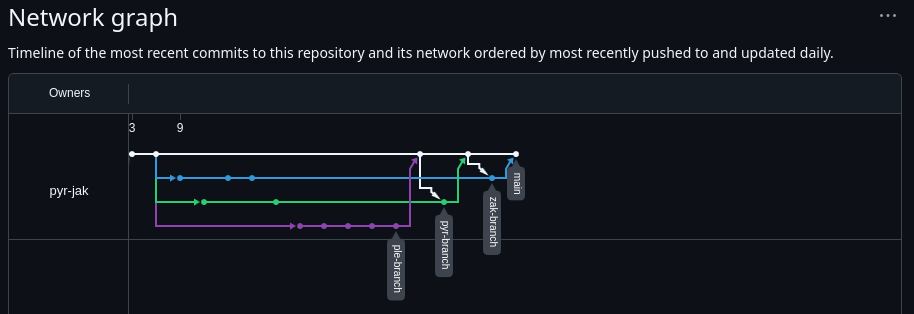
\includegraphics[width=\linewidth,height=0.40\textheight,keepaspectratio]{rys/network_graph.png}%
}{%
  \fbox{\parbox[c][0.20\textheight][c]{0.92\linewidth}{%
    \centering
    \textbf{Miejsce na zrzut ekranu z GitHub Network Graph}\\[4pt]
    \kod{rys/network_graph.png}%
  }}%
}
\caption{Historia gałęzi i punktów scalenia w widoku GitHub Network}
\label{rys:network-graph}
\end{figure}
